\chapter{The General Tab}

The General tab is responsible for displaying general information about the
current project.  Figure \ref{fig:general} shows the General tab displaying
information for the ``eugene\_gridcell'' project.  This information
includes a brief description of the project, the project name, the parent
project configuration, and a list of available datasets that can be used in
computing the values of expressions.  The ``parent'' field identifies the
XML project from which the currently open project inherits.  Inheritance is
described in further detail in Chapter \ref{chapter:xml-inheritance}.  Add
a dataset to the ``available\_datasets'' field if you have any extra
datasets to be added to the project.  The ``dataset\_pool\_configuration''
field includes a field named ``package\_order'' that gives the search order
when searching for variables implemented as Python classes; it is unlikely
that you'll want to change it.

The fields of the General tab can be edited by simply double clicking the
value side of a field that is part of a project.  If a field is displayed
in blue, this field is being inherited from the parent project, and must
first be added to the current project before editing can be done. To add a
field to the current project, right-click and select ``Add to current
project''.  Once added, the field may be edited as usual.

If you edit the ``parent'' field (not a typical operation), immediately
save and close the project, and then re-open it, so that the inherited
fields from the new parent will be shown

\begin{figure}[htp]
\begin{center}
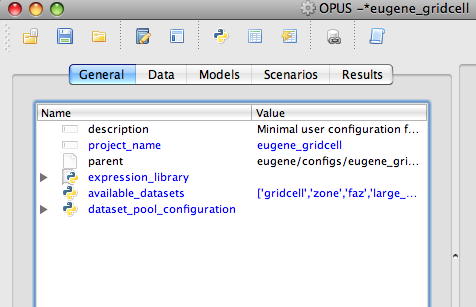
\includegraphics[scale=0.6]{part-gui/images/general-tab.png}
\end{center}
\caption{The General Tab}
\label{fig:general}
\end{figure}

